\chapter{Theory and Fundamentals of Array Processing and Beamfoming}

 A technique known as array processing is used to extract information from signals gathered by an array of sensors or antennas.This project aims to showcase a widely used technique for spatial filtering called beamforming, which uses an array of sensors to extract the desired signal that is spatially propagating from a specific direction and identify the strong interferences regions to generate low power and efficient  beam pattern.

\section{ Array fundamentals}

A spatially propagating signal may contain information about both its originating location and the material it is carrying. There are always undesired signals present in addition to the signal, such as noise and intentional and inadvertent interferences. A
single sensor can be used to separate the received signal into its multiple components as long as it has the ability to spatially discriminate the signals based on direction (at the very least). Directivity refers to a sensor’s capacity to spatially distinguish between different signal components received.\textbf{S. haykin} This ability depends on  the geometric structure’s shape and physical properties. Such a single-sensor system, however, has a number of shortcomings. The following are some drawbacks of single sensor/receiver elements:
\begin{itemize}
\item A receiver system based on a single receiver element, similar to a paraboloid dish element, produces a highly directed, high gain sensor with a particular radiation pattern. Every time the reception direction changes, the dish must be mechanically rotated to that precise location in the new direction.
\item The dwell time associated with mechanical rotation is noticeably long, which poses a significant challenge in an adaptive context where the signal circumstances are constantly changing.
\item A single sensor can only be appropriately positioned to receive signals from one direction if it is instantly focused at it; it cannot estimate the DOA of a signal. 
\end{itemize}
The Figure\ref{fig:idea} depicts the beam pattern formed by using an array of sensors that can address these single-sensor limitations, making it suited for many application constraints that single-sensor systems impose on receiver operability.
\begin{figure}[h]
\centering
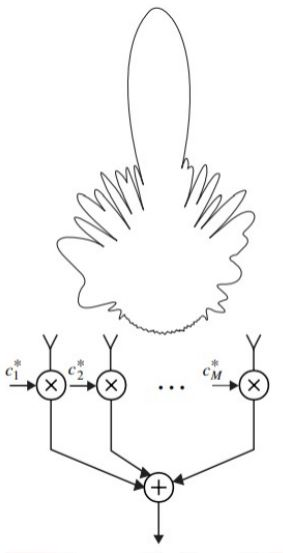
\includegraphics[scale=1]{Chapter2/Figures/idea}		
\caption{ \label{fig:idea}Beam Pattern}
\end{figure}

The sensor array's signals are combined so that one direction is highlighted while others are suppressed or not. The most significant advantage of arrays is that their focus or point can be directed in almost any direction, regardless of how they are arranged. The sensors can be connected in a variety of distinct ways to emphasize different orientations, each of which may carry a Signal of Interest (SoI). Because the various weighted summations of the sensors simply amount to processing the same data in different ways, these many sources can be received at the same time. Arrays can also change the total rejection level in specific directions to counteract a strong interference source.

\section{ Array Model}
The way the array of sensors spatially arranged have  a significant impact on the final beam pattern,which is a crucial factor in determining the array's directivity and performance.Array spacing determines the constructive and destructive interference patterns of the signals received or transmitted by the individual antennas. In this section, we will delve into the effects of different array spacing configurations on the resulting beam pattern, beam-width, side lobes, nulls, and overall directivity of the antenna array. Smaller spacing allows for a finer angular resolution, enabling more precise beam steering. On the other hand, wider spacing may limit the array's ability to steer the main lobe accurately.So the relationship between array geometry and beam pattern is essential for optimizing the array's performance for specific applications.
Various array geometries are commonly used in antenna arrays, each with unique characteristics.
\begin{itemize}
\item Uniform Linear Array (ULA): A linear arrangement of antennas with equal spacing between adjacent elements.Characteristics of the ULA beam pattern, including the main lobe width, side lobes, and nulls.
\item Uniform Rectangular Array (URA):An array with antennas arranged in a rectangular grid, with equal spacing in both the horizontal and vertical directions.
\item Uniform Circular Array (UCA):Antennas arranged in a circular pattern with equal spacing between antennas.Understanding the unique properties of the UCA beam pattern, including azimuthal symmetry.
\item Non-Uniform Array (NRA):An array with antennas placed irregularly, allowing for additional degrees of freedom in beam shaping.
\end{itemize}

\begin{figure}[h]
\centering
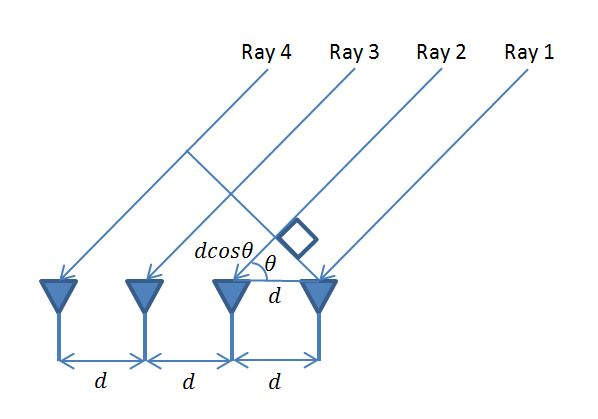
\includegraphics[scale=0.75]{Chapter2/Figures/array}		
\caption{ \label{fig:array}Array of sensors separated distance "d"}
\end{figure}
Figure\ref{fig:array} is an uniform linear array. Consider a single signal that is propagating and strikes the ULA at an angle $\phi$. Due to the fact that all of the elements are similarly spaced, the spatial signal has a difference in propagation pathways between any two sequential sensors of d sin($\phi$), resulting in a temporal delay.This separation and arrangement of  this array elements shows a significant impact on the final beam pattern analysed.
 
\section{Beamforming}
Beamforming is an advanced signal processing technique that is widely used in applications involving antenna or sensor arrays. It enables the manipulation and control of the array's radiation or reception pattern, resulting in better directional sensitivity and signal detection and estimation.Instead of uniformly radiating or receiving signals in all directions, beam forming concentrates the energy of the array in a specific direction while decreasing receptivity to signals from other directions. This capacity to selectively direct the array's beam provides considerable benefits in terms of enhanced SNR, interference rejection, and spatial selectivity.\\
The fundamental idea of beamforming is to modify the phase and amplitude of signals received or transmitted by individual array elements. By adjusting the phases and amplitudes of the signals, constructive interference occurs in the desired direction, amplifying the signal, while destructive interference occurs in other directions, reducing undesirable signals. This causes the array's emission or reception pattern to form a narrow and focussed main lobe, which can be electronically guided to track a target or optimize reception.\\
\subsection{Non Adaptive beamforming}
   Non-adaptive beamforming is a traditional beamforming technique used in antenna arrays and sensor arrays to create a fixed, predetermined beam pattern.Non-adaptive beamforming relies on carefully designing and setting the array's weights or coefficients to achieve a specific desired beam pattern. These weights are determined during the design phase and remain constant during signal processing. By controlling the phase and amplitude of the signals transmitted or received by each element in the array, non-adaptive beamforming creates a narrow main lobe in the desired direction, providing enhanced sensitivity to signals from that direction.This fixed beam pattern is particularly useful in applications where the array needs to maintain a steady direction of focus, such as in radar systems for tracking specific targets or in wireless communication systems for coverage in a specific direction.This are simple,easy and cost less to design but they lack adaptability which is essential for the modern applications.
\subsection{Adaptive beamforming}   
   Adaptive beamforming is a smart signal processing technique used in antenna arrays and sensor arrays to dynamically alter the weights or coefficients of the array based on the received data. 
This is achieved by iteratively updating the weights in response to the received signals. Adaptive algorithms use statistical properties of the received signals to estimate the optimal set of weights that maximize the array's directivity towards the desired signal while minimizing sensitivity to interference and noise.As the signal environment evolves, the array adapts its beam direction to track moving targets or to null out interference sources, resulting in enhanced performance and improved signal-to-interference-plus-noise ratio (SINR).
\begin{figure}[h]
\centering
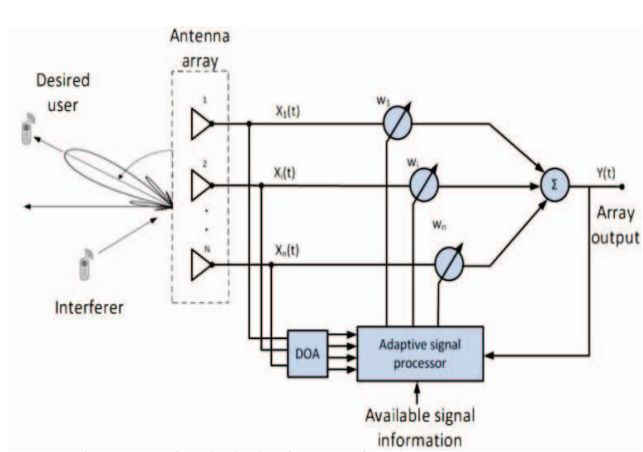
\includegraphics[scale=0.75]{Chapter2/Figures/1}		
\caption{ \label{fig:1}Adaptive Beamformer Design}
\end{figure} 

\section{Need of subarrays in Adaptive Beamforming}
 As discussed in the above sections when we use a array of sensors as a transmitter or a receiver we need to deal with a delay to achieve required beam pattern.In fixed beamformer its done by physically adjusting antenna elements and in adaptive beamformer an electronic unit(time delay units) adjusts this delays.So this electronic units makes adaptive beamforming algorithms can be computationally intensive, especially when applied to large-scale antenna arrays.To avoid this we can using simple phase shifter but they work efficiently fixed range of frequencies and introduces beam squints in the presences of other frequencies.So as a tradeoff we use both phase shifters and time units by using the concept of subarrays.\\
\begin{figure}[h]
\centering
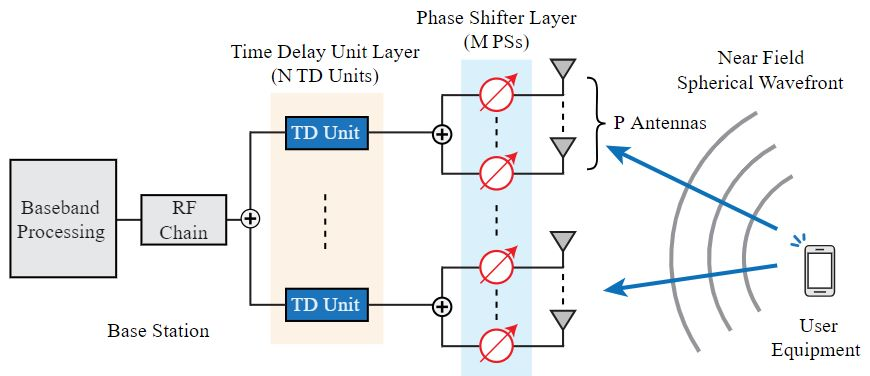
\includegraphics[scale=0.8]{Chapter2/Figures/1 main}		
\caption{ \label{fig:1}Adaptive beamforming using subarrays}
\end{figure} 

Subarrays provide additional degrees of freedom in beamforming design. By configuring multiple subarrays with varying positions, orientations, or element spacings, adaptive beamforming gains greater flexibility in shaping the beam pattern. This enhances the array's ability to track multiple targets simultaneously, adjust to non-stationary signals, and optimize performance for specific signal scenarios.\\
Subarrays are particularly useful in achieving adaptive nulling, where unwanted interference or jamming signals are suppressed. By configuring subarrays with spatial separation, adaptive algorithms can steer nulls toward interference sources while maintaining sensitivity to the desired signals. This results in improved interference rejection and a higher signal-to-interference-plus-noise ratio (SINR)  
 
\section{Use of Acronyms and Glossaries}
Acronyms are nothing but the short form of regular repeated word. Say for example, you have a repeat word "Integrated Circuits" and you want to use a short form for it as "IC". For which you have to first define the word and use it wherever you wanted to refer it.

First, let's look at the definition, which has to be entered in \texttt{Glossaries.tex} under \texttt{CoverPages} directory.
\begin{verbatim}
%\newacronym{<Ref>}{<Short-Form>}{<Expanded word>}
\newacronym{ic}{IC}{Integrated Circuits}
\end{verbatim}
In order to use the defined acronym, use the commands \verb|\gls{<Ref>}| as shown below

As an example, call the definition with \verb|\gls{ic}| and the outcome of it is reflected as, \gls{ic}.

Note: For the First time, the expanded form appears along with the Short-form definition inside parenthesis. But when the \verb|\gls{}| is repeated, only Short-form appears inside the parenthesis.

Now, let's look at the definition of symbols. Follow the syntax to define the symbol first, inside \texttt{Glossaries.tex} under \texttt{CoverPages} directory.
\begin{verbatim}
%\newglossaryentry{<Ref>}{name=<Symbol>, description={<description about the symbol>}, type=<List type>}
\newglossaryentry{rc}{name=$\tau$, description={Time constant}, type=symbolList}
\end{verbatim}

As an example, the rate of change is defined with \verb|\gls{rc}| and the outcome of it is reflected as, the rate of change is defined with \gls{rc}.

\vspace{0.75cm}

 \textbf{The chapters should not end with figures, instead bring the paragraph explaining about the figure at the end followed by a summary paragraph.}

After elaborating the various sections of the chapter (From Chapter 2 onwards), a summary paragraph should be written discussing the highlights of that particular chapter. This summary paragraph should not be numbered separately. This paragraph should connect the present chapter to the next chapter.